\section{\textbf{WAHRSCHEINLICHKEITSTHEORIE} - Ereignisse und Wahrscheinlichkeiten}
\subsection{Zufallsereignisse}
Der Ausgangspunkt jeder wahrscheinlichkeitstheoretischen Betrachtung ist ein Zufallsvorgang oder Zufallsexperiment (Würfeln, prüfen eines Werkstücks). Einen Zufallsvorgang zeichnet aus, dass es mehrere, \emph{sich gegenseitig ausschließende} Ergebnisse gibt, von dem genau eines Eintreten wird, wobei nicht bekannt ist welches. Die \emph{möglichen} Ergebnisse eines Zufallsvorgang werden mit $\omega$ und die Menge aller Ergebnisse d.h. der \emph{Ergebnisraum} werden als $\Omega$ bezeichnet. Beim Einmaligen Würfeln kann $\omega$  z.B. $\omega = \{2\}$ sein, während $\Omega = \{1, 2, 3, 4, 5, 6\}$ ist. Wenn man beim Würfeln eine 5 oder 6 benötigen um zu gewinnen, ist man daran interessiert, ob das
Ergebnis des Würfelwurfes in einer bestimmten Teilmenge von $\Omega$ liegt, konkret in der Menge $\{5, 6\}$. Diese Teilmengen nennt man \emph{(Zufalls-)Ereignisse} und man sagt, dass ein Ereignis $A \subset \Omega$ eintritt, wenn das Ergebnis $\omega$ des Zufallsvorgang ein Element von A is. Die einelementigen Teilmengen $\{\omega\}$ von $\Omega$ nennt man auch \emph{Elementareereignisse}.\\\\
\textbf{Mengenlehre und wahrscheinlichkeitstheoretische Interpretation}: \emph{Kommutativgesetz}: $A \cap  B = B \cap A$. \emph{Assoziativgesetz}: $(A \cap B ) \cap C = A \cap (B \cap C)$. \emph{Distributivgesetz}: $(A \cup B) \cap C = (A \cap C) \cup (A \cap C)$. \emph{De Morgansche Regel}: $\overline{(A \cap B)} = \bar{A} \cup \bar{B}$ (geht auch, wenn man $\cap$ und $\cup$ vertauscht)\\\\
\textbf{Ereignisfelder}: Die Menge aller Ergebnisse bezeichnet man als \emph{Ereignisfeld} $\mathcal{F}$. Wenn der Ergebnisraum $\Omega$ endlich oder abzählbar unendlich ist, ist die Potenzmenge $\mathcal{P}(\Omega)$ das üblicherweise betrachtete Ereignisfeld. Ist $\Omega$ überabzählbar können als Ereignisfelder nur $\sigma$-Algebren betrachtet werden. Diese sind definiert durch: $\Omega \in \mathcal{F}$,\,\,\,$A \in \mathcal{F} \Rightarrow \bar{A} \in \mathcal{F}$,\,\,\,abzählbar viele Ereignisse $A_1, A_2, ... \in \mathcal{F} \Rightarrow \cup_{i=1}^\infty A_i \in \mathcal{F}$

\subsection{Laplace-Wahrscheinlichkeiten und Kombinatorik}
\begin{wrapfigure}{r}{0.4\textwidth}
    \vspace{-6mm}
    \centering
    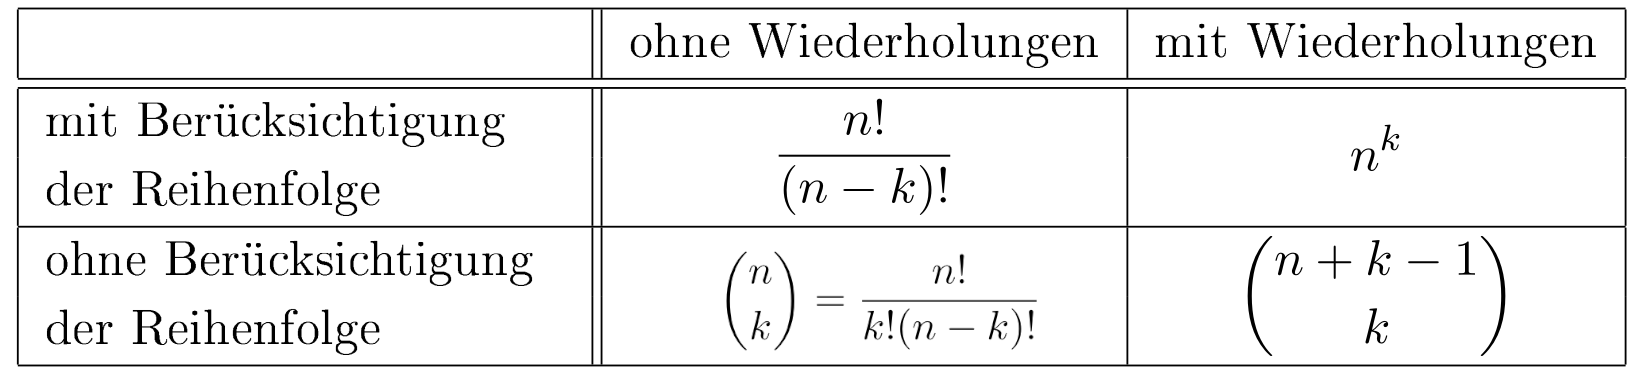
\includegraphics[width=0.4\textwidth]{images/wiederholung_kombinatorik.png}
    \caption{Kombinatorik Wiederholung}
    \vspace{-6mm}
    \label{fig:}
\end{wrapfigure}
\textbf{Laplace-Wahrscheinlichkeit}: $P(A) = \frac{\text{Anzahl der für $A$ günstigen Ergebnisse}}{\text{Anzahl aller möglichen Ergebnisse}} = \frac{|A|}{|\Omega|}$. Bsp. die Wahrscheinlichkeit eine ungerade Zahl zu würfeln: $P(A) = \frac{|\{1,3,5\}|}{|\{1,2,3,4,5,6\}|} = \frac{3}{6} = \frac{1}{2}$

\textbf{Permutation}: Anordnen von n unterscheidbaren Objekten: $n \cdot (n-1) \cdot (n-2) ... = \Pi_{i=1}^n i = n!$. Bsp: Sitzordnung an einem Tisch.\,\,\,\,\textbf{Variation ohne Wiederholungen}: Möglichkeiten k aus n unterscheidbaren Objekten \emph{mit} Berücksichtigung der Reihenfolge auszuwählen. Formel 1 Siegertreppchen Anordnungen bei 20 Teilnehmern.\,\,\,\,\textbf{Variation mit Wiederholungen}: Bsp. k mal ziehen aus n Möglichkeiten. Bsp: Kombinationen bei Passwörtern.\,\,\,\,\textbf{Kombination ohne Wiederholungen} Ziehen von k aus n Objekten. Die Reihenfolge spielt keine Rolle. Bsp: \hlc{Lotto} 6 aus 49.\,\,\,\,\textbf{Kombination mit Wiederholungen}: Die Anzahl Kombinationen beim Auswählen von k Objekten aus n unterscheidbaren Objekten.
\subsection{Wahrscheinlichkeitsmaße}
\textbf{Definition Wahrscheinlichkeitsmaß}: Es sei $\Omega$ der Ergebnisraum eines Zufallsvorgangs und $\mathcal{F}$ ein Ereignisfeld über $\Omega$. Eine Abbildung $P$ die jedem Ereignis $A \in \mathcal{F}$ eine reelle Zahl zuordnet: $P: \mathcal{F} \rightarrow \mathds{R}$ mit $A \mapsto P(A)$ nennt man \emph{Wahrscheinlichkeitsmaß} auf $\mathcal{F}$ wenn sie die \hlc{Axiome von Kolmogoroff} erfüllt: \textbf{K1} $P(A) \ge 0$ (Nichtnegativität).\,\,\,\,\textbf{K2} $P(\Omega) = 1$ (Normierung).\,\,\,\,\textbf{K3} Falls $A \cap B = \emptyset$, so ist $ (A \cup B) = P(A) + P(B)$ (Additivität).\\
Daraus folgen folgende Rechenregel:\,\,\,\,(\textbf{i}) $0 \le P(A) \le 1$.\,\,\,\,(\textbf{ii}) $P(\emptyset) = 0$.\,\,\,\,(\textbf{iii}) $P(A) \le P(B)$, falls $A \subset B$.\,\,\,\,(\textbf{iv}) $P(\bar{A}) = 1 - P(A)$.\,\,\,\,(\textbf{v}) $P(A_1\cup ... \cup A_k) = P(A_1) + ... + P(A_k)$ falls $A_1, ..., A_k$ paarweise disjunkt. $\Rightarrow$ $P(A) = \sum_{w \in A}P(\{\omega\}.$\,\,\,\,(\textbf{vi}) $P(B \backslash A) = P(B) - P(A \cap B)$.\,\,\,\,(\textbf{vii}) $P(A\cup B) = P(A) + P(B) - P(A \cap B)$ (Additionssatz)
\subsection{Bedingte Wahrscheinlichkeiten und unabhängige Ereignisse}
Die Wahrscheinlichkeit eines Ereignisses ändert sich möglicherweise, wenn wir zusätzlich Information in Form des Eintritts eines anderen Ereignisses erhalten. Wahrscheinlichkeit für Pünktlichkeit sinkt bei Stau. Die Definition der \hlc{bedingten Wahrscheinlichkeit} ergibt sich hierbei Analog zur relativen Häufigkeitsverteilung: \hlcm{$P(A|B) = \frac{P(A \cap B)}{P(B)}$}. Bsp: Wie hoch ist die Wahrscheinlichkeit eine 6 zu würfeln unter der Bedingung, dass die gewürfelte Zahl gerade ist? Antwort: $P(A|B) = \frac{P(\{6\} \cap \{2,4,6\})}{P(\{2,4,6\})} = \frac{1/6}{3/6} = \frac{1}{3}$\\
\begin{wrapfigure}{l}{0.25\textwidth}
    \vspace{-6mm}
    \centering
    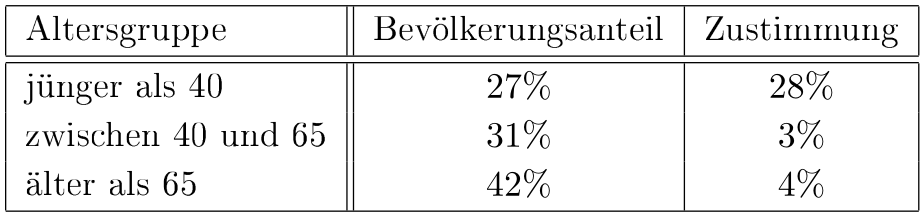
\includegraphics[width=0.25\textwidth]{images/beispiel_wahl_satz_der_tot_wahscheinlichkeit.png}
    \caption{Eine Partei hat analysiert, wie ihre Demographie ist.}
    \vspace{-5mm}
    \label{fig:pool_total}
\end{wrapfigure}
Der \hlc{Produktsatz} garantiert, dass für zwei Ergebnisse $A$ und $B$ mit $P(B) > 0$ gilt: \hlcm{$P(A \cap B) = P(B) \cdot P(A|B)$}. Diese Aussage gilt auch im allgemeinen für $A_1, ..., A_n$ mit $P(A_1 \cap ... \cap A_n) > 0$:\\$P(\cap_{i=1}^nA_i) = P(A_1) \cdot P(A_2|A_1) \cdot P(A_3|A_1 \cap A_2) \cdot P(A_n|A_1 \cap ... \cap A_{n-1}) = P(A_1) \cdot \Pi_{i=2}^n P(A_i|A_1 \cap ... \cap A_{i-1})$. \hlc{Stochastiche Unabhängikeit} bedeutet wenn sich die Wahrscheinlichkeit eines Ereignisses $A$ beim Eintritt eines anderen Ereignisses $B$ \emph{nicht} ändert. Sprich $P(A|B) = P(A)$. Somit gild dann mit dem Produktsatz $P(A \cap B) = P(B) \cdot P(A | B) = P(B) \cdot P(A)$. Dies gilt Analog für $n$ Ereignisse. \hlc{Satz der totalen Wahrscheinlichkeit}: Sei $A_1, ..., A_n$ eine disjunkte Zerlegung des Ereignisraums $\omega$ mit $P(A_j) > 0$, $j = 1, ..., n$. Dann gilt für ein weiteres Ereignis $B$: \hlcm{$P(B) = \sum_{j=1}^nP(B|A_j) \cdot P(A_j)$}. Bsp Wahl (vgl \cref{fig:pool_total}) Welchen Stimmanteil hat die Partei insgesamt bekommen? Antwort: $P(B) = \sum_{j=1}^3 = P(B|A_j) \cdot P(A_j) = 0.28 \cdot 0.27 + 0.03 \cdot 0.031 + 0.04 \cdot 0.42 = 0.1017$. \hlc{Satz von Bayes}: Sei $A_1, ..., A_n$ eine disjunkte Überdeckung des Ereignisses $B$ und $P(A_j) > 0$ sowie $P(B|A_j) > 0$ für mindestens ein $j = 1, ..., n$. Dann gilt: \hlcm{$P(A_j|B) = \frac{P(B|A_j) \cdot P(A_j)}{P(B)} = \frac{P(B|A_j) \cdot P(A_j)}{\sum_{i=1}^nP(B|A_i) \cdot P(A_i)}, j = 1, ..., n$}. Dieser Satz überträgt die \emph{a-priori} Wahrscheinlichkeit $P(A_j)$ in eine \emph{a-posteriori} Wahrscheinlichkeit $P(A_j|B)$. Bsp. Wie groß ist die Wahrscheinlichkeit, dass ein Wähler zur Gruppe \glqq jünger als 40\grqq\, gehört? Antwort: ($P(B)$ wurde mit Satz der tot. Wahrscheinlichkeit berechnet) $P(A_1|B) = \frac{P(B|A_1) \cdot P(A_1)}{P(B)} = \frac{0.28 \cdot 0.27}{0.1017}$
\section{Zufallsvariablen}
\begin{wrapfigure}{r}{0.2\textwidth}
    \vspace{-10mm}
    \centering
    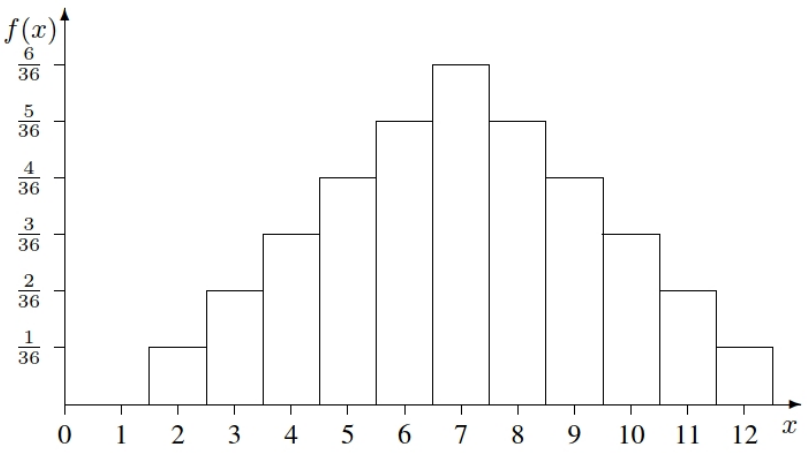
\includegraphics[width=0.2\textwidth]{images/5.1_f_augensumme.png}
    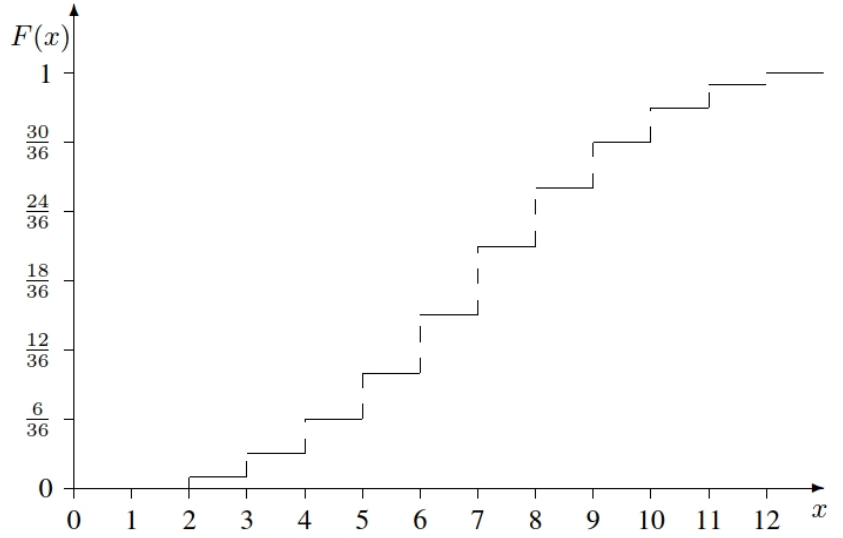
\includegraphics[width=0.2\textwidth]{images/5.2_F_augensumme.png}
    \caption{Wahrscheinlichkeitsion (oben) und Verteilungsfunktion für die Augensummen bei zweimaligen Würfeln.}
    \vspace{-3mm}
    \label{fig:f_F_dice}
\end{wrapfigure}
Bei der Beobachtung oder Durchführung von Zufallsvorgängen ist man häufig gar nicht an den Ergebnissen selbst interessiert, sondern an daraus abgeleiteten Größen. Beim zweimaligen Würfeln könnte dies beispielweise die Summe der Augenzahlen sein. Hier besteht der Ereignisraum $\Omega$ aus 36 Zahlenpaaren $\omega = (i, j)$ mit $1 \le i,j \le 6$, relevant ist für jedes Zahlenpaar aber nur die Information $i + j$. Durch die Zuordnung der reellen Zahl $i + j$ zu jedem Ergebnis $\omega = (i, j)$ erhält man eine \emph{Zufallsvariable}. Wenn wir $X$ für die Augensumme der zwei Würfe verwenden erhalten wir also die Zuordnung bzw. Abbildung $X: \omega = (i, j) X(\omega) = X(i, j) = i + j$. Diese Schreibweise ermöglicht es Ereignisse sehr knapp und einfach zu Formulieren. So entspricht dem Ereignis \glqq die Augensumme ist 4\grqq\, kurz \{$X=4$\} was ausführlich $\{X = 4\} = \{\omega \in \Omega: X(\omega) = 4 = \{(1,3), (2,2), (3,1)\}$ bedeutet. 
\section{Diskrete Zufallsvariablen}
Eine Zufallsvariable heißt diskret, wenn sie nur endlich oder abzählbar unendlich viele Werte annehmen kann, d.h. $W(X) = \{x_1, x_2, ...\}$. Die Wahrscheinlichkeitsverteilung ist dann gegeben durch $P(X = x_i) = p_i$ eindeutig festgelegt. Nach dem ersten Axiom von Kolmogoroff ist $0 \le p_i \le 1$ und die Wahrscheinlichkeit für ein Ereignis $\{X \in A\}$ mit $A \subset W(X)$ ist $P(X \in A) = \sum_{i:x_i \in A} p_i$. Nach dem zweiten Axiom von Kolmogoroff folgt damit sofort $\sum_{i \ge 1} p_i = P(X \in W(X)) = 1$. Die Wahrscheinlichkeitsverteilung ist Analog zur relativen Häufigkeitsverteilung. Während die Wahrscheinlichkeitsverteilung die möglichen Ausgänge eines Zufallsvorgangs theoretisch beschreibt basiert die relative Häufigkeitsverteilung auf tatsächlichen Beobachtungen in einer Stichprobe.
\hlc{Definition Wahrscheinlichkeitsfunktion.}: \hlcm{$f(x) = f_X() := \begin{cases}
    P(X = x_i) = p_i &\text{, }x = x_i \in W(X)\\
    0 &\text{, sonst.}
\end{cases}$}. $W(X)$ sei hierbei der Wertebereich einer Zufallsvariable X.
Die \hlc{Verteilungsfunktion} ist \hlcm{$F(x) = F_X(x) := P(X\le x) = \sum_{i: x_i \le x}f(x_i) = \sum_{i: x_i \le x} p_i$}. Die Verteilungsfunktion ist insbesondere zur \hlc{Berechnung von Wahrscheinlichkeiten der Form $P(a < X \le b)$} mit $a, b \in \mathds{R}$ und $a < b$ hilfreich, denn es gilt \hlcm{$P(a < X \le b) = F(b) - F(a)$}\\\\
\hlc{Unabhänigkeit diskreter Zufallsvariablen}: $n$ Diskrete Zufallsvariablen $X_1, .., X_n$ heißen stochastisch unabhängig, wenn für beliebige $x_1 \in W(X_1), ..., x_n \in W(X_n)$ gilt: $P(X_1 = x_1, ..., X_n = x_n) = P(X_1 = x_1) \cdot ... \cdot P(X_n = x_n)$. Anschaulich: Für das Würfeln von zwei Würfeln  $X_1$ und $X_2$ mit zwei beliebigen Augenzahlen $i$ und $j$ gilt: $P(X_1 = i, X_2 = j) = \frac{1}{36} = \frac{1 \cdot 1}{6 \cdot 6} = P(X_1 = i) \cdot P(X_2 = j)$.


\subsection{Maßzahlen diskreter Wahrscheinlichkeitsverteilungen}
\hlc{Erwartungswert einer Diskreten Zufallsvariable}: Sei $X$ eine diskrete Zufallsvariable mit Wertebereich $W(X) = \{x_1, x_2, ...\}$ und Wahrscheinlichkeitsverteilung $p_1, p_2, ...$. Dann ist der Erwartungswert von $X$:\\ \hlcm{$E(X) := \sum_{i\ge1} x_i \cdot p_i = \sum_{i\ge1} x_i \cdot f(x_i) = \mu_x = \mu$}. Eigenschaften: \textbf{1} Für eine Funktion $g: \mathds{R} \rightarrow \mathds{R}$ ist auch $Y = g(X)$ eine Zufallsvariable, und zwar mit Wahrscheinlichkeitsverteilung $P(Y = y) = \sum_{i: g(x_i) = y} p_i$. \textbf{2} Der Erwartungswert von $Y$ ist dann $E(Y) = E(g(X)) = \sum_{i\ge1} g(x_i) \cdot p_i = \sum_{i\ge1} g(x_i) f(x_i)$. \textbf{3} Im Spezialfall einer linearen Transformation $g(x) = ax + b$ ist $E(Y) = E(aX+b) = aE(X) + b$. \textbf{4} Für Zufallsvariablen $X_1, ..., X_n$ und Konstanten $a_1, ..., a_n \in \mathds{R}$ gilt $E(a_1X_1 + ... + a_nX_n) = a_1E(X_1) + ... + a_nE(X_n)$. \textbf{5} Für unabhängige Zufallsvariablen $X_1$ und $X_2$ gilt außerdem $E(X_1 \cdot X_2) = E(X_1) \cdot E(X_2)$\\\\
\hlc{Modus disktrer Zufallsvariablen} Jede lokale Maximumstelle der Wahrscheinlichkeitsfunktion $f_X(x)$ einer diskreten Zufallsvariablen $X$ ist ein Modus $x_{mod}$ der Verteilung von $X$. Bsp. Lokales Maximum in \cref{fig:f_F_dice} (oben) ist $x_{mod}$.\\\\
\hlc{Varianz und Standardabweichung diskreter Zufallsvariablen} Sei $X$ eine diskrete Zufallsvariable mit Wertebereich $W(X) = \{x_1, x_2, ...\}$ und Wahrscheinlichkeitsverteilung $p_1, p_2$. dann ist die Varianz von $X$: $\sigma_x^2 = \sigma^2 = Var(X):= $ $ :=\sum_{i\ge1} (x_i - E(X))^2 \cdot p_i = \sum_{i\ge1} = (x_i - E(X))^2 \cdot f(x_i)$ dementsprechend ist die Varianz \hlcm{$\sigma = \sqrt{Var(X)}$}. Bei der praktischen Berechnung ist der \emph{Verschiebungssatz} recht hilfreich: \hlcm{$Var(X) = E(X^2) - (E(X))^2$}. Eigenschaften der Varianz: \textbf{1} Die Varianz der transformierten Y(X) = g(X) als reelle Funktion ist $Var(Y) = Var(g(X)) = \sum_{i\ge1} [g(x_i) - E(g(X))]^2 \cdot p_i = \sum_{i\ge1} [g(x_i) - E(g(X))]^2 \cdot f(x_i) = E[(g(X) - E(g(X)))^2] = E(g(X)^2) - E^2(g(X))$. \textbf{2} Im Spezialfall einer lin. Transformation $g(x) = ax + b$  ist $Var(Y) = Var(aX + b) = a^2Var(X)$ damit folgt für die Stdabw. $\sigma_Y = |a|\sigma_x$. \textbf{3} Für unabhängige Zufallsvariablen $X_1, ..., X_n$ und Konst. $a_1, ..., a_n \in \mathds{R}$ gilt: $Var(a_1X_1 + ... + a_nX_n) = a_1^2Var(X_1) + ... + a_n^2Var(X_n)$ 
\newpage
\subsection{Konkrete diskrete Wahrscheinlichkeitsverteilungen}
\, % wichtig für plot
\begin{wrapfigure}{l}{0.21\textwidth}
    \vspace{-7mm}
    \centering
    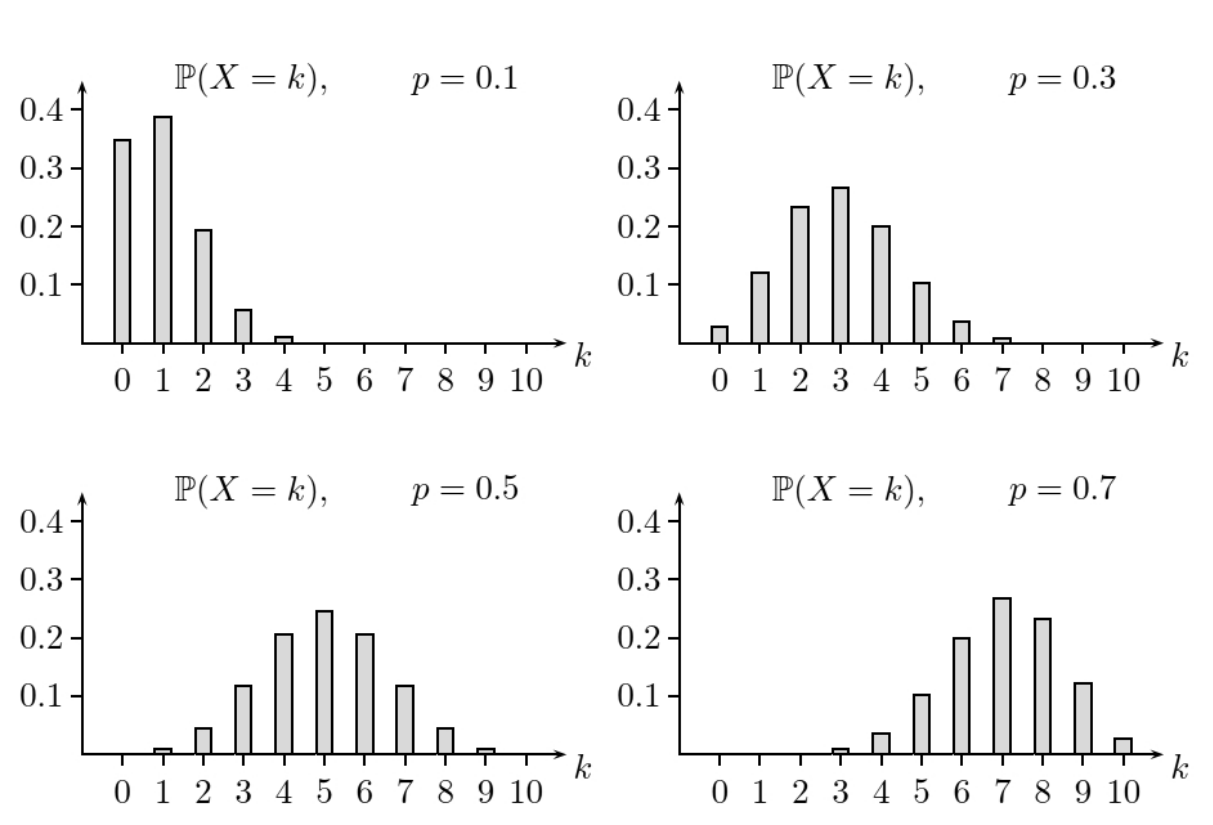
\includegraphics[width=0.21\textwidth]{images/5.3 Wahrscheinlichkeitsverteilungen bin(10,p).png}
    \includegraphics[width=0.21\textwidth]{images/5.5 Wahrscheinlichkeitsverteilungen poi(λ).png}
    \includegraphics[width=0.21\textwidth]{images/5.6 Wahrscheinlichkeitsverteilungen geo(λ).png}
    \caption{Bin(10, p) (oben), Poi($\lambda$), Geo(p)}
    \vspace{-26mm}
    \label{fig:disk_dist}
\end{wrapfigure}
\hlc{Diskrete Gleichverteilung} Eine diskrete Zufallsvariable heißt gleich- oder Laplace-verteilt, wenn alle möglichen Werte mit gleicher Wahrscheinlichkeit auftreten. Wahrscheinlichkeitsfunktion: $f(x) = \begin{cases}
    \frac{1}{n}&x\in W(X)\\
    0&\text{sonst}
\end{cases}$. Erwartungswert: $E(X) = \frac{1}{n}\sum_{i=1}^nx_i$. Varianz: $Var(X) = E(X^2) - (E(X))^2 = \frac{1}{n}\sum_{i=1}^nx_i^2 - \frac{1}{n^2}(\sum_{i=1}^nx_i)^2$. \emph{Mögliche Anwendungen:} Münzwurf, Würfel. \\\\
\hlc{Bernoulli-Verteilung - $X \sim Ber(p)$} Einen Zufallsvorgang, der nur zwei mögliche Ergebnisse hat. In der Regel geht es um die Frage, ob ein bestimmtes Ereignis A eintritt oder nicht. $W(X) = \{0,1\}$. \hlc{$p = P(A)$}. Wahrscheinlichkeitsverteilung: $p_0 = P(X=0) = 1 - p$ und $p_1 = P(X=1) = p$. $E(X) = p$ und $Var(X) = p(1-p)$. \emph{Mögliche Anwendungen:} Qualitätsprüfung (Bauteil besteht oder nicht)\\\\
\hlc{Binomialverteilung - $X \sim Bin(n, p)$ / $X \sim B(n, p)$} Erweiterung der Bernoulli-Verteilung. Man führt ein Bernoulli-Experiment \hlc{$n$}-Mal durch. Wahrscheinlichkeit für $k$ von $n$ erfolgreiche Versuche: $p_k = \binom{n}{k} p^k  (1-p)^{n-k}, k = 0, ..., n$. Wahrscheinlichkeitsfunktion $f(X) = P(X = x) = \begin{cases}
    \binom{n}{x} p^x  (1-p)^{n-x} & x = 0, 1, ..., n\\
    0 & \text{sonst}
\end{cases}$. Erwartungswert $E(X) = np$. $Var(X) = np(1-p)$. Gilt $X \sim Bin(n, p)$ und $Y \sim Bin(m, p)$ so gilt $X + Y \sim Bin(n + m, p)$. \emph{Mögliche Anwendungen:} Modellierung der Wahrscheinlichkeit, dass ein Byte Korrekt übertragen wird.\\\\
\hlc{Poisson-Verteilung - $X \sim Poi(\lambda)$} Modelliere Anzahl von Ereignissen in begrenzten Zeitraum. $W(X) = \mathds{N}_0$. Annahmen: \textbf{1} Zwei Ereignisse können nicht gleichzeitig auftreten. \textbf{2} Die Wahrscheinlichkeit für ein Ereignis Wächst proportional mit der Länge des betrachteten Zeitabschnitts. \textbf{3} Die \emph{Wahrscheinlichkeit} für eine bestimmte Anzahl Ereignisse hängt nur von der Länge des betrachteten Zeitintervalls ab, nicht von dessen Lage. Für tatsächliche Beobachtungen gilt das natürlich nicht. \textbf{4} Die Anzahl von Ereignissen in zwei disjunkten Zeitintervallen sind unabhängig. Wahrscheinlichkeitsfunktion: $f(x) = P(X=x) = \begin{cases}
    \frac{\lambda^x}{x!}e^{-\lambda} & x \in \mathds{N}_0\\
    0 & text{sonst}
\end{cases}$. $E(X) = \lambda$ $Var(X) = \lambda$. $X \sim Poi(\lambda)$ und $Y \sim Poi(\mu)$ $\Rightarrow$ $X + Y \sim Poi(\lambda + \mu)$ \emph{Mögliche Anwendungen} Reaktorüberwachung. 5 Ereignisse pro Tag. Wie hoch ist die Wahrscheinlichkeit für mehr als Zehn? $\rightarrow$ $P(N > 10) = \sum_{k=11}^\infty p_k = 1 - \sum_{k=0}^{10}p_k$ \\\\
\hlc{Geometrische Verteilung - $X \sim Geo(p)$} Zum modellieren der Anzahl an notwendiger Wiederholungen bis zum erstmaligen Eintritt des erwarteten Ereignisses. Sei $X$ die Anzahl \emph{unabhängiger} Versuchswiederholungen bis zum erstmaligen Eintritt des Ergebnisses $A$ und \hlc{$p = P(A)$}. Die Wahrscheinlichkeitsfunktion lautet $f(X) = P(X = x) = \begin{cases}
    (1 - p) ^ (k-1) p & x \in \mathds{N}\\
    0 & \text{sonst}
\end{cases}$. $E(X) = \frac{1}{p}$. $Var(X) = \frac{1-p}{p^2}$. Außerdem Verteilungsfunktion für $x \ge 0$: $F(x) = P(X \le x) = P(X \le \lfloor x\rfloor) = 1 - (1 - p)^{\lfloor x\rfloor}$



\section{Stetige Zufallsvariablen}
\subsection{Definition und Unabhängigkeit}
\,
\begin{wrapfigure}{r}{0.2\textwidth}
    \vspace{-20mm}
    \centering
    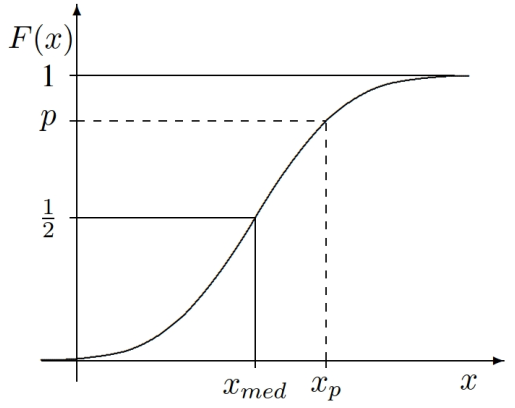
\includegraphics[width=0.2\textwidth]{images/6.4_1.png}
    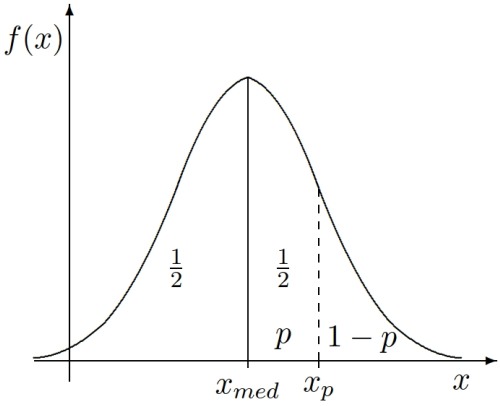
\includegraphics[width=0.2\textwidth]{images/6.4_2.png}
    \caption{Verteilungsfunktion (oben) Wahrscheinlichkeitsdichtefunktion (unten).}
    \vspace{-10mm}
    \label{fig:stetig_f_F}
\end{wrapfigure}
\hlc{Stetige Zufallsvariablen und Wahrscheinlichkeitsdichte} Eine Zufallsvariable $X$ heißt stetig, wenn es eine Funktion $f(x)$ gibt, sodass für jedes Intervall $[a, b] \subset \mathds{R}$ gilt: $P(a \le X \le b) = \int_a^b f(x) dx$. Die Funktion $f(x) = f_X(x)$ heißt Wahrscheinlichkeitsdichtefunktion (oder Dichtefunktion ) von $X$. Aus der Definition folgt, das die Wahrscheinlichkeit einen konkreten Wert $a$ zu beobachten, null ist, denn $P(X = a) = \int_a^a f(x) dx = F(a) - F(a) = 0$ für alle $a\in\mathds{R}$. Daraus kann man $P(a \le X \le b) = P(a < X \le b) = P(a \le X < b) = P(a < X < b)$ ableiten. Aus den \emph{Axiomen von Kolmogoroff} ergeben sich dann noch, dass die Dichte $f(X) \ge 0$ für alle $x \in \mathds{R}$ (bis auf abzählbar viele Ausnahmen) sein muss und \emph{normiert} sein muss: $P(X \in \mathds{R}) = \int_{-\infty}^\infty f(x)dx = 1$ \\\\
Durch die Wahrscheinlichkeitsdichte ist auch die \hlc{Verteilungsfunktion} einer stetigen Zufallsvariablen eindeutig bestimmt: $F(X) = P(X \le x) = \int_{-\infty}^x f(u) du$. Sie besitzt folgenden Eigenschaften: \textbf{1} F(X) ist stetig, monoton wachsen mit $W(F(x)) \in [0, 1]$. \textbf{2} Das Grenzverhalten ist wie im diskreten Fall $\underset{x \rightarrow -\infty}{\text{lim}}F(x) = 0$ und $\underset{x \rightarrow \infty}{\text{lim}}F(x) = 1$. \textbf{3} Wenn die Dichte $f(x)$ an der STelle $x$ stetig ist, gilt $F'(x) = f(x)$. \textbf{4} Für $a, b \in \mathds{R}$ gilt \hlcm{$P(a \le X \le b) = P(a < X \le b) = P(a \le X < b) =$ $= P(a < X < b) = F(b) - F(a)$} und \hlcm{$P(X \ge a) = P(X > a) = 1 - P(X \le a) = 1 - F(a)$} \\\\
\hlc{Unabhängigkeit stetiger Zufallsvariablen} Analog zur Unabhängigkeit diskreter Zufallsvariablen sind auch stetige Zufallsvariablen $X_1, ..., X_n$ unabhängig, wenn für beliebige Mengen $A_1, ..., A_n \subset \mathds{R}$ gilt: $P(X_1 \in A_1, ..., X_n \in A_n) = P(X_1 \in A_1) \cdot ... \cdot P(X_n \in A_n)$. Dies gilt sobald die Gleichheit für alle Mengen der Form $A_i = (-\infty, x_i]$ gegeben ist.
\subsection{Maßzahlen stetiger Wahrscheinlichkeitsverteilungen}

Sei $X$ eine stetige Zufallsvariable mit Wahrscheinlichkeitsdichte $f(x)$ Dann ist der \hlc{Erwartungswert} von $X$ $E(X):=\int_{-\infty}^\infty x\cdot f(x)dx$ \textbf{vorgesetzt} $\int_{-\infty}^\infty |x|\cdot f(x)dx < \infty$. Eigenschaften des Erwartungswert: \textbf{1} Für eine Funktion $g: \mathds{R} \rightarrow \mathds{R}$ besitzt die Zufallsvariable $Y = g(X)$ den Erwartungswert $E(Y) = E(g(X)) = \int_{-\infty}^{\infty}g(x) \cdot f(x) dx$. \textbf{2} Wenn g(x) linear dann $E(Y) = aE(X) + b$. \textbf{3} Ist die Dichte symmetrisch um den Punkt $c$, also $f(x - x) = f(c + x)$ für alle $x$, so ist $E(X) = c$. \textbf{4} Für Zufallsvariable $X_1, ..., X_n$ und Konstanten $a_1, ..., a_n \in \mathds{R}$ gilt $E(a_1X_1 + ... + a_nX_n) = a_1E(X_1) + ... + a_nE(X_n)$. \textbf{5} Für unabhängige Zufallsvariable $X_1$ und $X_2$ gilt außerdem $E(X_1 \cdot X_2) = E(X_1) \cdot E(X_2)$. \hlc{Modus} analog zu diskreten Zufallsvariablen.\\
\hlc{p-Quantil}: Das $p$-Quantil mit $0<p<1$ zu einer Zufallsvariablen $X$ ist ein Wert $x_p$, den die Zufallsvariable mit einer Wahrscheinlichkeit von $p \cdot 100\%$ \emph{unterschreitet} und mit einer Wahrscheinlichkeit von $(1 - p) \cdot 100\%$ \emph{überschreitet}: $P(X \le x_p) = p$ und $P(X \ge x_p) = 1 - p$. Per Definition ist das $p-Quantil$ jeder Wert $x_p$ für den gilt \hlcm{$F(x_p) = P(X \le x_p) = p$}. Der \hlc{Median} ist dann der Wert $x_{med}$ für $p = 0.5$. Es gilt \hlcm{$F(x_{med}) = 0.5$}\\
\hlc{Varianz und Standardabweichung}: Sei $X$ eine stetige Zufallsvariable mit Wahrscheinlichkeitsdichte $f(x)$, dann ist die Varianz von $X$ $\sigma^2 = Var(X):= \int_{-\infty}^{\infty}(x - E(X))^2 \cdot f(x) dx$. Die Standardabweichung ist wiederum \hlcm{$\sigma = \sqrt{Var(X)}$}. Praktisch wird die Varianz analog zum diskreten Fall mit dem Verschiebungssatz bestimmt \hlcm{$\sigma^2 = Var(X) = E(X^2) - E^2(X)$}. Eigenschaften der Varianz: \textbf{1} Die Varianz kann als Erwartungswert einer geeignet transformierten Zufallsvariable geschrieben werden: $Var(X) = E[(X - E(X))^2]$. \textbf{2} Die Varianz der transformierten Zufallsvariable $Y = g(X)$ mit $g(x)$ als reeler Funktion ist $Var(Y) = Var(g(X)) = \int_{-\infty}^{\infty}[g(x_i) - E(g(X))]^2 \cdot f(x) dx = E[(g(X) - E(g(X)))^2] = E(g^2(X)) - E^2(g(X))$ für $g(x) = ax + b$ ist $Var(Y) = Var(aX + b) = a^2Var(X)$ und $\sigma_Y = |a|\sigma_X$. \textbf{4} Für \emph{unabhängige Zufallsvariablen} $X_1, ..., X_n$ und Konstanten $a_1, ..., a_n \in \mathds{R}$ gilt $Var(a_1X_1 + ... + a_nX_n) = a_1^2Var(X_1) + ... + a_n^2Var(X_n)$\\\\
\hlc{Zentrierung und Standardisierung} Eine Zufallsvariable $X$ heißt \emph{zentriert}, wenn $\mu = E(X) = 0$ ist. Sie heißt \emph{standardisiert}, wenn zusätzlich $\sigma^2 = Var(X) = 1$ ist. Für jede Zufallsvariable $X$, für die Erwartungswert $\mu$ und Varianz $\sigma^2$ existieren, erhält man mit Hilfe der linearen Transformation \hlcm{$Z = \frac{X - \mu}{\sigma}$}, denn $E(Z) = E(\frac{X - \mu}{\sigma}) = \frac{1}{\sigma}(E(X) - \mu) = 0$ und $Var(Z) = Var(\frac{X - \mu}{\sigma}) = \frac{1}{\sigma^2} Var(X) = 1$. Die Standardisierung ist vor allem für die Normalverteilung sehr wichtig.
\subsection{Konkrete Wahrscheinlichkeitsverteilungen}
\,
\begin{wrapfigure}{l}{0.15\textwidth}
    \vspace{-7mm}
    \centering
    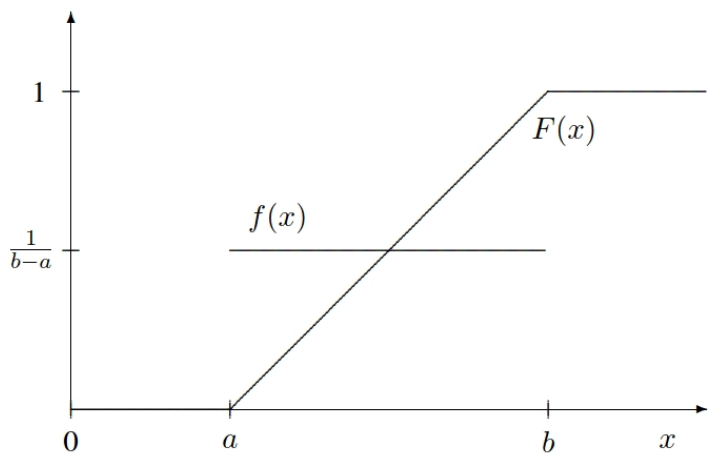
\includegraphics[width=0.15\textwidth]{images/6.5_f_F_stetige_gleichverteilung.png}
    \caption{Stetige Gleichverteilung}
    \vspace{-14mm}
    \label{fig:stetige_gleichverteilung_f_F}
\end{wrapfigure}
\hlc{Stetige Gleichverteilung - $X \sim U(a, b)$} Wahrscheinlichkeitsdichte ist konstant auf einem reellen Intervall \hlc{$[a, b]$}. Aufgrund der Normierungseigenschaft gilt für die Dichte: $f(x) = \begin{cases}
    \frac{1}{b-a} & \text{, }a \le x \le b\\
    0 & \text{, sonst}
\end{cases}$ und für die Verteilungsfunktion: \\$F(x) = \begin{cases}
    0 & x < a\\
    \frac{x-a}{b-a} & a\le x \le b\\
    1 & x > b
\end{cases}$ Der Erwartungswert und Varianz sind $E(X) = \frac{a + b}{2}$ und $Var(X) = \frac{(b - a)^2}{12}$. \emph{Mögliche Anwendungen}: Modellierung einer Bruchstelle in einer Wasser- oder Stromleitung, oder die Generierung von Zufallszahlen.\\\\
\hlc{Exponentialverteilung - $X \sim Exp(\lambda)$}:
Die Exponentialverteilung ist das stetige Analogon zur geometrische Verteilung. Eine stetige Zufallsvariable $X$ heißt exponentialverteilt mit Parameter $\lambda > 0$, wenn die Wahrscheinlichkeitsdichte folgende Form hat: $f(x) = \begin{cases}
    \lambda e^{-\lambda x} & \text{, } x \ge 0\\
    0 & \text{, sonst.}
\end{cases}$ Der Parameter \hlc{$\lambda$} wird als (Ausfall-)Rate bezeichnet. Die Verteilungsfunktion lautet $F(X) = \begin{cases}
    1 - e^{-\lambda x} & \text{, } x \ge 0\\
    0 & \text{, sonst}
\end{cases}$ Erwartungswert und Varianz sind $E(X) = \frac{1}{\lambda}$ und $Var(X) = \frac{1}{\lambda^2}$
Zusammenhang zw. Exponential- und Poisson-Verteilung: Sei N die Anzahl Ereignisseintritte in einem fest definierten Zeitintervall und seien $T_1, T_2, ...$ die Zeitdauern zwischen aufeinander folgenden Ereignisseiftritten. Dann gilt $N \sim Poi(\lambda) \Leftrightarrow T_1, T_2, ... \sim Exp(\lambda)$ und unabhängig. 
\emph{Mögliche Anwendungen}: Modellierung von Zeitdauern. Zum Beispiel die Länge von Telefonaten oder Lebensdauern von Produkten sowie die Bearbeitungszeit von Aufträgen.\\\\
\hlc{Normalverteilung - $X \sim N(\mu, \sigma^2)$} Eine Zufallsvariable $X$ heißt normalverteilt mit parametern $\mu \in \mathds{R}$ und $\sigma^2 > 0$, wenn sie die Wahrscheinlichkeitsdichte $f(x) = \frac{1}{\sqrt{2\pi}\sigma} e^{-\frac{(x - \mu)^2}{2\sigma^2}}$, $x \in \mathds{R}$. \hlc{$E(X) = \mu$}. \hlc{$Var(X) = \sigma^2$}. Die Verteilung ist symmetrisch d.h. $f(\mu - x) = f(\mu + x)$. \emph{Die Verteilungsfunktion der Normalverteilung kann nicht analytisch bestimmt werden.}\\\\
\hlc{Standardnormalverteilung - $X \sim N(0, 1)$}: $f(x) = \frac{1}{\sqrt{2\pi}} e^{-\frac{x^2}{2}}$ die Verteilungsfunktion $\phi(z)$ mit $z \ge 0$ muss in Tabellen nachgeschlagen werden! Negative werte können mit $\phi(-z) = 1 - \phi(z)$. \hlc{Umrechnung mittels Standardisierung:} Wenn $X \sim N(\mu, \sigma^2)$, dann gilt $Z = \frac{X - \mu}{\sigma}$ konkret: $F(x) = P(X \le x) = P(\frac{X - \mu}{\sigma} \le \frac{x - \mu}{\sigma}) = \phi(\frac{x - \mu}{\sigma})$. \hlc{Quantile}: $\phi(z_p) = p$, $0 < p < 1$ für $p < 0.5$ ist $z_p = -z_{1-p}$. Rücktransformation: $x_p = \sigma z_p + \mu$.
\hlc{zentrale Schwakungsintervalle}: ein symmetrisches Intervall um den Erwartungswert, in dem eine Größe mit einer bestimmten Wahrscheinlichkeit liegt. Konkret ein Intervall der Form $[\mu - c, \mu + c]$ mit $c > 0$ mit einer konkreten Wahrscheinlichkeit $0 < \alpha < 1$. c ist dann so zu wählen, dass $P(\mu - c \le X \le \mu + c) = P(|X - \mu| \le c) = 1 - \alpha$, d. h. $c = z_{1 - \frac{\alpha}{2}} \sigma$. \hlc{$k\sigma$-Bereiche der Normalverteilung}: Anschaulich bedeutet dies, dass eine Größe ein $k$-faches um ihre Standardabweichung schwankt: $[\mu - k\sigma, \mu + k\sigma] k\in \mathds{N}$. $k = 1$: $P(\mu - \sigma \le X \le \mu + \sigma) = P(|X - \mu| \le \sigma) = 0.6827$ analog für $P(|X - \mu| \le 2\sigma) = 0.9545$ bzw. $P(|X - \mu| \le 3\sigma) = 0.9973$.\\
\hlc{Rechenregeln}: \textbf{1} Für $X \sim N(\mu, \sigma^2)$ und $Y = a X + b$ mit $a, b \in \mathds{R}$ und $a \neq 0$ ist die Verteilung $Y \sim N(a\mu + b,a^2 \sigma^2)$. \textbf{2} Sind $X \sim N(\mu_X, \sigma_X^2)$ und $Y \sim N(\mu_Y, \sigma_Y^2)$ so ist $X + Y \sim N(\mu_X + \mu_Y, \sigma_X^2 + \sigma_Y^2)$ (lässt sich auf n \emph{unabhängige} Zufallsvariablen erweitern).\\\\
\hlc{Lognormalverteilung - $X \sim N(\mu, \sigma^2)$} Genau so, wie $N(\mu, \sigma^2)$, nur dass man $ln$ auf Eingangswerte anwenden muss. $E(X) = e^{\mu + \sigma^2/2}$ und $Var(X) = e^{2\mu + \sigma^2}(e^{\sigma^2} - 1)$ \emph{Mögliche Anwendungen}: Einkommen, Wartezeit, Versicherungsschaden, Niederschlagsmengen, Wachstumsfaktoren.\\\\

\hlc{$\chi^2$ Verteilung - $Z \sim \chi^2(n)$}: Seien $X_1, ..., X_n$ unabhängige standardnormalverteilte Zufallsvariablen d.h. $X_i \sim N(0, 1)$. Dann folgt die Zufallsvariable $Z = X_1^2 + ... + X_n^2$. \hlc{n} bezeichnet die Freiheitsgrade. $E(Z) = n$ und $Var(Z) = 2n$. Quantile: $\chi_p^2(n)$ für $n \le 30 \rightarrow$ Tabellen. Annäherung für $n > 30$: $\chi_p^2(n)=0.5(z_p + \sqrt{2n - 1})^2$  \emph{Mögliche Anwendungen}: Für kleine $n$ ist die Verteilung rechtsschief und daher für die Modellierung von Lebensdauern Geeignet.Wird $n$ größer nähern  sich die Dichten der Normalverteilungsdichte an.\\
\hlc{Student's $t$-Verteilung - $T \sim t(n)$}: Seien $X \sim N(0, 1)$ und $Z \sim \chi^2(n)$ unabhängige Zufallsvariablen. Dann folgt die Zufallsvariable $T = \frac{X}{\sqrt{Z/n}}$. $E(T) = 0$ für $n \ge 2$ und $Var(T) = \frac{n}{n-2}$ für $n \ge 3$. \emph{Mögliche Anwendungen}: Für kleine $n$ deutlich \glqq spitzer\grqq\, als $N(\mu, \sigma^2)$. Kann für dinge verwendet werden, die weniger um $\mu$ schwanken. Läuft aber gegen eine Normalverteilung für große $n$\\
$\chi^2$ und Students's $t$-Verteilung: Verteilungen, die nur selten zur Modellierung konkreter Sachverhalte verwendet werden. Sie dienen insbesondere als \emph{Testverteilungen} in der induktiven Statistik. Dabei wird anhand ihrer Quantile beurteilt, mit welcher Hypothese zutreffen ist oder nicht.

\section{Gesetz der großen Zahlen und zentraler Grenzwertsatz}
\subsection{Gesetz der großen Zahlen}
\hlc{Schwaches Gesetz der großen Zahlen}: Seien $X_1, X_2, ...$ unabhängige Zufallsvariablen mit Erwartungswert $\mu$ un nach oben beschränkten Varianzen, d.h. $\sigma_1^2, \sigma_2^2 \le s$ für ein fixes $s > 0$. Dann gilt für ein beliebiges $\epsilon > 0$: $P(|\bar{X}_n - \mu| \le \epsilon) \rightarrow 1$. Man sagt, dass $\bar{X}_n$ \emph{in Wahrscheinlichkeit gegen $\mu$ konvergiert}\\\\
\hlc{Theorem von Bernoulli (empirisches Gesetz der großen Zahlen)}: Die relative Häufigkeit, mit der ein Ereignis $A$ bei $n$ unabhängigen Wiederholungen eines Zufallsvorgangs eintritt, konvergiert in Wahrscheinlichkeit gegen $P(A)$. \\\\
\hlc{Satz von Gilvenko-Cantelli (Hauptsatz der Statistik)}: Seien $X_1, X_2, ...$ unabhängige und identisch verteilte Zufallsvariablen mit Verteilungsfunktion $F(x)$. Außerdem sei $F_n(x)$ die aus $X_1, ..., X_n$ abgeleitete empirische Verteilungsfunktion. Dann gilt für ein beliebiges $\epsilon > 0$: $P({\underset{x\in \mathds{R}}{sup} | F_n(x) - F(x)| \le \epsilon}) \rightarrow 1$ für $n \rightarrow \infty$
\subsection{Zentraler Grenzwertsatz}
\hlc{Definition}:Seien $X_1, X_2, ...$ unabhängige und identisch verteilte Zufallsvariablen mit endlichem Erwartungswert $E(X_i) = \mu$ und endlicher $Var(X_i) = \sigma^2$. Dann konvergiert die Verteilungsfunktion $F_n(z) = P(Z_n \le z)$ von $Z_n$ für $n \rightarrow \infty$ an jeder Stelle $z \in \mathds{R}$ gegen die Verteilungsfunktion $\phi(z)$ der Standardnormalverteilung $F_n(z) \rightarrow \phi(z)$ für $n \rightarrow \infty$\\
Wenn die Verteilung von $S_n$ bzw. $Z_n$ gegen eine Normalverteilung konvergiert, muss die Verteilung für große $n$ einer Normalverteilung bereits sehr ähnlich sein. Auch aus dem \emph{Zentralen Grenzwertsatz} folgt also, dass die Summe einer hinreichend großen Anzahl $n$ von unabhängigen Zufallsvariable einer beliebigen Verteilung (mit endlichem Erwartungswert $\mu$ und endlicher Varianz $\sigma^2$) durch eine Normalverteilung $N(n\mu, n\sigma^2)$ approximiert werden kann. Man schreibt kurz $S_n = X_1 + ... + X_n \overset{a}{\sim} N(n\mu, n\sigma^2)$ bzw. $Z_n \overset{a}{\sim} N(0, 1)$ und für die Verteilungsfunktion von $S_n$ gilt dann: $F_{S_n}(x) = P(S_n \le x) = P(\frac{S_n - n\mu}{\sqrt{n}\sigma} \le \frac{x - n\mu}{\sqrt{n}\sigma}) = P(Z_n \le \frac{x - n\mu}{\sqrt{n}\sigma}) \approx \phi(\frac{x - n\mu}{\sqrt{n}\sigma})$
\emph{Mögliche Anwendung}: n Personen warten auf Auf Ereignis wie bsp check-in.\\\\
\hlc{Grenzwertsatz von de Moivre}: Für ein hinreichend großes $n$ kann die Binomialverteilung $Bin(n, p)$ durch eine $N(np, np(1-p))$ Verteilung approximiert werden.\\\\
\hlc{Approximation der Poisson-Verteilung}: Für ein hinreichend großes $\lambda$ kann die Poisson-Verteilung $Poi(\lambda)$ durch $N(\lambda, \lambda)$ approximiert werden. Lambda sollte so groß sein, damit die Poisson-Verteilung annähern symmetrisch ist.\\\\

% \section{Zufallsvektoren}